Quando aplicamos uma janela $w[n]$ ao sinal, o sinal janelado é dado por:
$$
   x_w[n] = x[n] \cdot w[n]
$$
onde $w[n]$ é uma função de janela de tamanho $N$, usada para minimizar os efeitos de vazamento espectral. Exemplos comuns de janelas incluem a janela de Hamming, Hann, e retangular.

A DTFT do sinal janelado, $X_w(e^{j \omega})$, é dada pela convolução da DTFT do sinal original $X(e^{j \omega})$ com a DTFT da janela $W(e^{j \omega})$:
$$
   X_w(e^{j \omega}) = X(e^{j \omega}) * W(e^{j \omega})
$$

\subsection*{DTFT do Sinal Sem Janela}

Para referência, a DTFT do sinal original $x[n] = C + A \cos(2 \pi \alpha n)$ (sem janela) pode ser calculada como a soma das DTFTs de cada termo:

1. \textbf{DTFT da componente DC} $C$:
$$
   X_{\text{DC}}(e^{j \omega}) = C \cdot 2 \pi \delta(\omega)
$$

2. \textbf{DTFT da componente cossenoidal} $A \cos(2 \pi \alpha n)$:

Podemos expressar o cosseno em termos de exponenciais complexas:
$$
   A \cos(2 \pi \alpha n) = \frac{A}{2} \left( e^{j 2 \pi \alpha n} + e^{-j 2 \pi \alpha n} \right)
$$
Assim, a DTFT dessa parte é:
$$
   X_{\cos}(e^{j \omega}) = \frac{A}{2} \cdot 2 \pi \left( \delta(\omega - 2 \pi \alpha) + \delta(\omega + 2 \pi \alpha) \right)
$$

3. \textbf{DTFT do sinal total} $x[n]$:
$$
   X(e^{j \omega}) = C \cdot 2 \pi \delta(\omega) + \frac{A}{2} \cdot 2 \pi \left( \delta(\omega - 2 \pi \alpha) + \delta(\omega + 2 \pi \alpha) \right)
$$

\subsection*{DTFT do Sinal Janelado}

Quando a janela $w[n]$ é aplicada, o espectro do sinal janelado $X_w(e^{j \omega})$ é a convolução do espectro do sinal $X(e^{j \omega})$ com o espectro da janela $W(e^{j \omega})$:
$$
   X_w(e^{j \omega}) = X(e^{j \omega}) * W(e^{j \omega})
$$

\subsection*{Computacionalmente}
No Octave, aplicamos a função da FFT para obter uma aproximação da DTFT, como mostra o exemplo abaixo.

\lstinputlisting[language=Octave]{02_analytic_development/example_fft.m}
\begin{figure}[H]
   \centering
   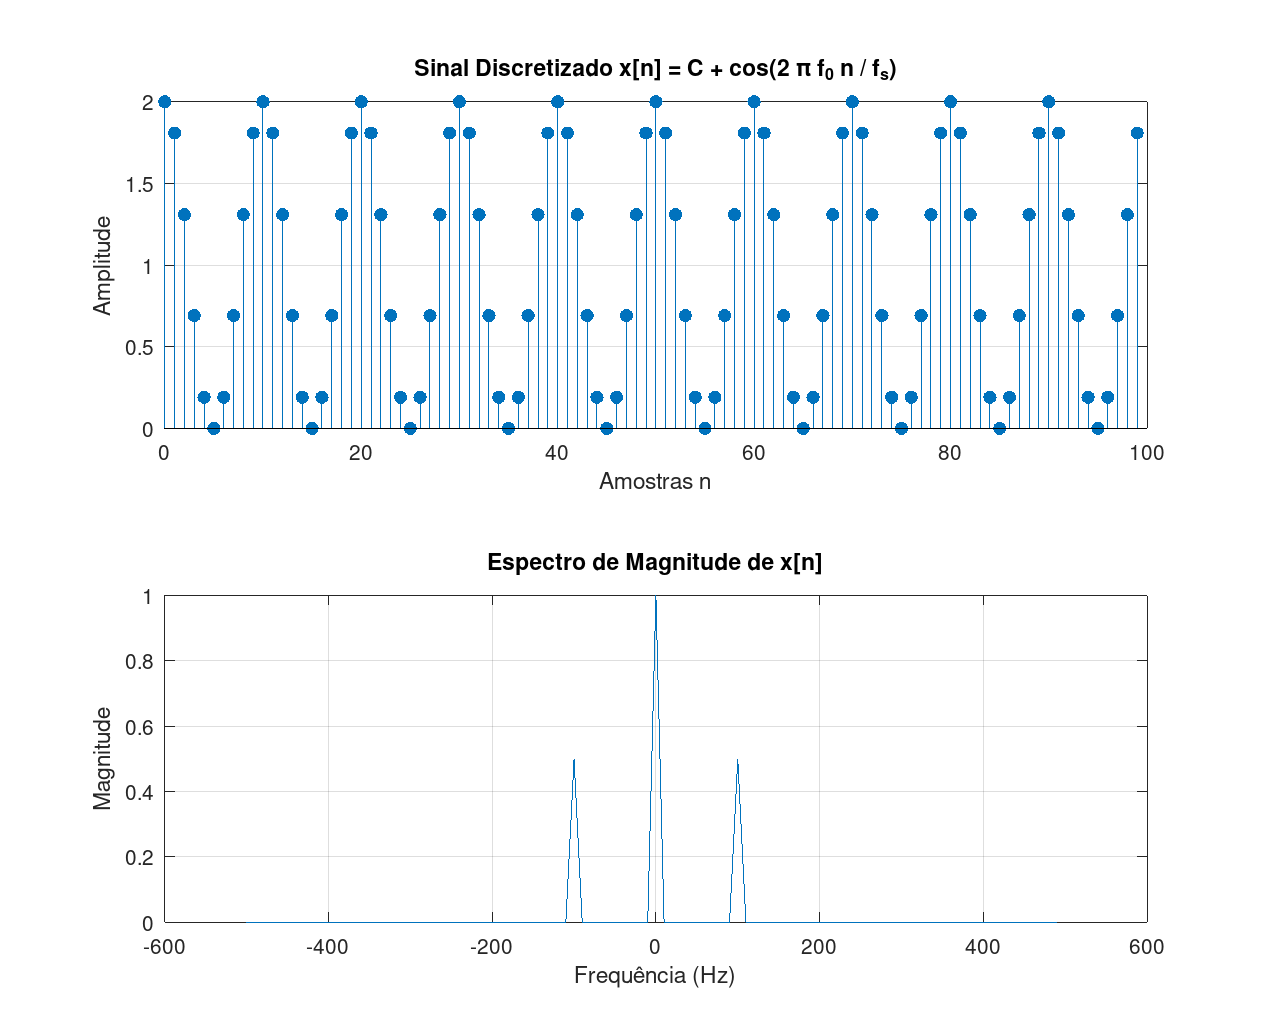
\includegraphics[width=1\linewidth]{02_analytic_development/example_fft.png}
   \caption{Sinal e Espectro de Magnitude}
   \label{fig:enter-label}
\end{figure}
